\documentclass{article}%[journal]{IEEEtran}
\usepackage{graphics,graphicx,subfigure,color}
\usepackage{calrsfs}
\usepackage{tikz} % graphical models
\usetikzlibrary{chains,fit,shapes}
\usetikzlibrary{bayesnet}
\usepackage{amsmath}
\usepackage{amsfonts}

\begin{document}

\title{Gibbs Sampling for Latent Dirichlet Allocation}

\author{Ali Caner T\" urkmen, G\" okhan \c Capan}
\date{}

% make the title area
\maketitle

\section{Introduction}
A plausible way to model sets of discrete variables, such as, a document of occurring words, log data associated to a person, and so on, is via mixed membership. In these models, we assume an overall membership proportion parameter for the set. Later, we say that each observed element comes from a multinomial distribution indexed by its latent, membership variable. This latent variable is drawn from the membership proportion parameter. 

Latent Dirichlet Allocation \cite{blei2003lda} is a way to model these kinds of data (and various related models exist, perhaps most notably nonnegative matrix factorization\cite{cemgil2009nmf}). In a Bayesian Network representation, the graphical model is as follows:
\begin{figure}[h]
	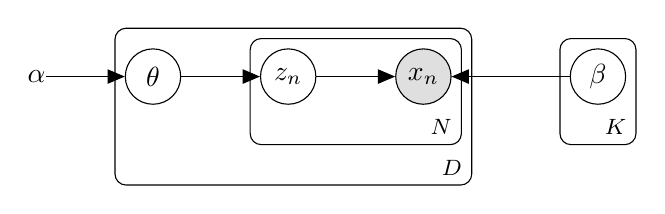
\begin{tikzpicture}
	  \node[latent] (z) {$z_n$} ; %
	  \node[obs, right = of z] (x) {$x_n$};
          \node[latent, left=of z] (theta) {$\theta$} ; %
          \node[const, left=of theta](alpha){$\alpha$};
          \node[latent, right=1.5 of x] (beta) {$\beta$};
        
          \edge {theta} {z} ; %
          \edge {z} {x} ;
          \edge {beta}{x} ;
          \edge {alpha}{theta}
          
          \plate {words}{
          	(z)
		(x)
	  }{$N$}
	  
          \plate {docs} {
          	(theta)
		(words)
          }{$D$}
          
          \plate {topicwords}{
          	(beta)
	 }{$K$}
    
	\end{tikzpicture}
	\end{figure}
\\The generative model describing the graphical representation:
	\begin{enumerate}
		\item For a set (of discrete observations);
		\begin{enumerate}
			\item Membership proportions vector is drawn ($\theta \sim Dirichlet(\alpha)$)
			\item For each observation (an element of the set)
			\begin{enumerate}
				\item Membership variable is drawn ($z_n \sim Multinomial(\theta)$)
				\item The discrete observation is drawn from ($x_n \sim Multinomial(\beta_{z_n})$)
			\end{enumerate}
		\end{enumerate}
	\end{enumerate}
	


\section{Posterior Probability of  $\theta$s and $z$s}
Treating $\beta$ as fixed for now, the posterior distribution for $\theta$s and $z$s is:
\begin{equation*}
P(\theta, z|x, \alpha, \beta) = \frac{P(\theta, z, x|\alpha, \beta)}{P(x|\alpha, \beta)}
\end{equation*}
The joint distribution (for a single set) in the nominator is:
\begin{equation*}
P(\theta, z, x|\alpha, \beta) = \frac{\Gamma(\sum_{i=1}^K \alpha_i)}{\prod_{i=1}^K\Gamma(\alpha_i)} \left(\prod_{i=1}^K \theta_i^{\alpha_i -1} \right) \left(\prod_{n=1}^N P(z_n|\theta)\prod_{j=1}^{|
\mathcal{X}|}\beta_{ij}^{[x_n = j]}\right)
\end{equation*}
And the evidence (denominator) can be written as:
\begin{equation*}
P(x|\alpha, \beta) = \frac{\Gamma(\sum_{i=1}^K \alpha_i)}{\prod_{i=1}^K\Gamma(\alpha_i)} \int d\theta \left(\prod_{i=1}^K \theta_i^{\alpha_i -1} \right) \left(\prod_{n=1}^N\sum_{i=1}^K\prod_{j=1}^V(\theta_i\beta_{ij})^{[x_n = j]}\right)
\end{equation*}
where we denote the set of observed variables ($\{x_n| x_n\in \mathcal{X}\}$) of size $N$ with $x$. $K$ is the number of possible \textit{clusters} that we assume (a hyperparameter of the model) a-priori. We sum over all $z_n$s and integrate over $\theta$ to get the evidence.

The normalizing constant is an intractable integral. This is the probability of observing a set, it allows us to assess our model's plausibility, which is much of interest. Further, if we want to make predictions, i.e., when we want to find next most probable element to the set (so that questions of kind \textit{what is this person going to do next? what other word can this document include?} can be answered), we need the posterior probability. The predictive distribution is as the following:
\begin{equation*}
P(x_{new}|x, \alpha, \beta) = \int d\theta \sum_z P(x_{new}|z, \beta_z), P(z, \theta|x, \alpha, \beta)
\end{equation*}

\section{Sampling From $z$s and $\beta$s}
Let $z$ be the sequence of membership variables, indexed in the same way with $x_n$'s associated with (the elements) a set $x$. Computing $P(z|x, \alpha, \beta)$ helps with prediction: We later can find $P(z_{new}|z)$. Given its $z_{new}$, the possible observation is independent from the membership proportions, so we can compute the predictive distribution by simply combining $P(z_{new}|z)$ with associated $\beta$. Computing $P(z|x, \alpha, \beta)$ requires integrating out $\theta$ from the posterior distribution. Here we will show how to integrate out $\theta$ from the joint  $P(z, x, \theta|\alpha, \beta)$ (avoiding the intractable normalizing constant), and then we will use the fact that $P(z, x|\alpha, \beta) \propto P(z|\alpha, \beta)$ to sample from $z$ \textit{a posteriori}. Recall that $z$ is multinomial, and a straightforward way to sample from it is with Gibbs Sampling, and the approach we take here, by integrating out $\theta$ is known as \textit{Collapsed Gibbs Sampling}.

The derivations are partly due to Wikipedia entry for Latent Dirichlet Allocation\footnote{https://en.wikipedia.org/wiki/Latent\_Dirichlet\_allocation\#Inference}. Let's first write $P(z, x|\alpha, \beta)$. We will denote number of assignments in the set to a cluster $i$ with $N_i$:
\begin{align*}
P(z, x|\alpha, \beta) =& \int d\theta P(\theta|\alpha) \prod_{n=1}^{N} P(z_n |\theta) P(x_n|\beta_{z_n}) d\theta\\
=&  \prod_{n=1}^{N} P(x_n|\beta_{z_n})  \int d\theta P(\theta|\alpha) \prod_{n=1}^{N} P(z_n |\theta) d\theta\\
=&  \prod_{n=1}^{N} P(x_n|\beta_{z_n}) \int d\theta \frac{\Gamma(\sum_{i=1}^K \alpha_i)}{\prod_{i=1}^K \Gamma(\alpha_i)}  \prod_{i=1}^K\theta_i^{\alpha_i - 1} \prod_{n=1}^N \prod_{i=1}^K \theta_i^{[z_n = i]}\\
=& \prod_{n=1}^{N} P(x_n|\beta_{z_n})   \int d\theta \frac{\Gamma(\sum_{i=1}^K \alpha_i)}{\prod_{i=1}^K \Gamma(\alpha_i)} \prod_{i=1}^K\theta_i^{\alpha_i - 1} \prod_{i=1}^K \theta_i^{N_i}\\
=& \prod_{n=1}^{N} P(x_n|\beta_{z_n})  \int d\theta \frac{\Gamma(\sum_{i=1}^K \alpha_i)}{\prod_{i=1}^K \Gamma(\alpha_i)}  \prod_{i=1}^K \theta_i^{N_i + \alpha_i -1}\\
\end{align*}
Notice that if we had $\frac{\Gamma(\sum_{i=1}^K N_i + \alpha_i)}{\prod_{i=1}^K \Gamma(N_i + \alpha_i)}$ instead of $\frac{\Gamma(\sum_{i=1}^K \alpha_i)}{\prod_{i=1}^K \Gamma(\alpha_i)}$, the term inside the integral would be a \textit{Dirichlet} pdf, and the result of integration would be 1. Using this, 
\begin{align*}
P(z, x|\alpha, \beta) =& \prod_{n=1}^{N} P(x_n|z_n, \beta) \frac{\Gamma(\sum_{i=1}^K \alpha_i)}{\prod_{i=1}^K \Gamma(\alpha_i)}  \frac{\prod_{i=1}^K \Gamma(N_i + \alpha_i)}{\Gamma(\sum_{i=1}^K N_i + \alpha_i)}\\
\end{align*}

Now that we integrated out $\theta$ and got $P(z, x|\alpha, \beta)$, we can use it to sample from $P(z_{n^\prime}|z_{\not n^\prime}, x, \alpha, \beta)$. Considering only the terms that depend on $z_{n^\prime}$;

\begin{equation*}
P(z_{n^\prime}|z_{\not n^\prime}, x, \alpha, \beta) \propto \beta_{z_{n^\prime}, x_{n^\prime}}  \prod_{i=1}^K \Gamma(N_i + \alpha_i)
\end{equation*}

Let's assume that we want to find the probability $P(z_{n^\prime} = k|z_{\not n^\prime}, x, \alpha, \beta)$. We can then decompose the above equation into:
\begin{align*}
P(z_{n^\prime} = k|z_{\not n^\prime}, x, \alpha, \beta) \propto& \beta_{k, x_{n^\prime}}  \prod_{i=1}^K \Gamma(N_i + \alpha_i)\\
=&\beta_{k, x_{n^\prime}}  \Gamma(N_k + \alpha_k)\prod_{i\neq k} \Gamma(N_i + \alpha_i)
\end{align*}
Excluding $z_{n^\prime}$ from the $\Gamma$ function, we have:
\begin{align*}
P(z_{n^\prime} = k|z_{\not n^\prime}, x, \alpha, \beta) \propto&\beta_{k, x_{n^\prime}}  \Gamma(N_k + \alpha_k)\prod_{i\neq k} \Gamma(N_i + \alpha_i)\\
=& \beta_{k, x_{n^\prime}} (N_k -1 +\alpha_k ) \Gamma(N_k -1 + \alpha_k)\prod_{i\neq k} \Gamma(N_i + \alpha_i)\\
\end{align*}
Since we excluded $z_{n^\prime}$, now both $\Gamma$ functions are just constants, and we have:
\begin{equation*}
P(z_{n^\prime} = k|z_{\not n^\prime}, x, \alpha, \beta) \propto \beta_{k, x_{n^\prime}} (N_k - 1 + \alpha_k)
\end{equation*}

An iteration of the Gibbs Sampler is by sampling from the above distribution for each element in the set, repeatedly in turn.

Recall that we treated $\beta$ as constant, but usually we also don't know it. A$\beta_k$ is a parameter of a multinomial over $\mathcal{X}$, and it can conveniently be modelled as $\beta \sim Dirichlet(\gamma)$. It can also be integrated out, and then we only sample $z_n$s. The derivation is almost analogous to what we did in integrating out $\theta$s, and we only show the resulting update rule for completeness (following \cite{griffiths2004collapsed}):

\begin{equation*}
P(z_{n^\prime} = k|z_{\not n^\prime}, x, \alpha, \beta) \propto \frac{C_{k,v}  -1 + \gamma_{v}}{\sum_{ v^{\prime} \in \mathcal{X}}C_{k,v^{\prime}} - 1 + \gamma_{v^{\prime}}} (N_k - 1 + \alpha_k)
\end{equation*}

where $C_k$ is a vector of counts over the entire data set (not for a single set as we write when we were deriving the sampling rules for $z_n$'s), $C_{k,v}$ being number of times $v\in \mathcal{X}$ is assigned to cluster $k$. Here, $v$ is whatever $x_{n^\prime}$ is. 

Alternatively, we can sample from $\beta_k$s. The previously derived sampling rule for $z_{n^\prime} = k|z_{\not n^\prime}, x, \alpha, \beta$s equally applies to sampling from  $z_{n^\prime} = k|z_{\not n^\prime}, x, \alpha, \beta$ in that case ($ \propto \beta_{k, x_{n^\prime}} (N_k - 1 + \alpha_k).
$). Sampling from $\beta_k|x,z,\alpha,\gamma$ is trivial: given everything, $\beta_k \sim Dirichlet(\gamma + C_k)$. This is because observing a $z_n = k$ allows us \textit{selecting} the $\beta_k$, and ignoring $\beta_{i}$s ($i\neq k$). 

One reason for \textit{not} collapsing $\beta_k$s might be that it makes $z$ updates independent. When sampling, following the order of first sampling all$z$s and then sampling $\beta$s makes the algorithm somewhat suitable to distributed processing environments such as  MapReduce (\cite{dean2008mapreduce}): sampling $z_n$'s, for each set, can be performed in parallel in the \textit{map} phase. Then we can sample from $\beta$ in the \textit{reduce} phase. This approach is also mentioned in \cite{newman2009distributed}. This procedure might be an option when the number of sets (documents, for instance) is huge, or already partitioned. Notice, however, its also introduces a communication cost: counts calculated by the independent processes should be accumulated to sample from $\beta$s. Additionally, this is expected to converge slower (in terms of iterations) than the fully collapsed sampler. This is also what we find in our experiments. In the latter case, we update the counts in place. There are, of course, other alternatives to implement LDA efficiently in a distributed environment, such as \cite{newman2009distributed, smyth2009asynchronous}. They vary in their approaches of making distributed computations more efficient: leveraging sparsity of data, careful partitioning of data so that the communication is minimal,  asynchronous updates from local counts, and so on. 

Finally, we write here a third alternative way of Gibbs Sampler update rules: sampling all $z_n$s, $\theta$s, and $\beta$s (nothing is integrated out):
\begin{align*}
z_{n^\prime}|z_{\not n^\prime},\theta,\beta \sim& P(z_{n^\prime}|\theta) P(x_{n^\prime}|z_{n^\prime}, \beta) \\
\theta|Z, \beta \sim& Dirichlet(\alpha + [N_1, N_2, \dots N_K])\\
\beta_k|Z, \theta \sim& Dirichlet(\gamma + C_k)\\
\end{align*}

The Monte Carlo estimate for $P(z_n)$'s and $P(\beta_k)$s are the empirical averages of our samples.

\subsection{Experiments}
We implemented the 3 variants of the Gibbs sampler (collapsed, non-collapsed, $\theta$-collapsed) as described in the previous section. The experiments are conducted on synthetic data, top-down sampled from the described generative model. What we report is the evidence, the joint probability of sets (the denominator of the posterior). We report the algorithm listings and the results in the poster. 
\bibliography{bibl}
\bibliographystyle{plain}

% that's all folks
\end{document}


